%harihiom
\documentclass{llncs}

\usepackage[english]{babel}
%\usepackage[utf8]{inputenc}
%\usepackage{amsmath}
\usepackage{graphicx}
\usepackage{float}
%\usepackage{wrapfig}
%\usepackage{titlepic}
%\usepackage[colorinlistoftodos]{todonotes}
\usepackage{graphicx,epstopdf}
\usepackage{amsmath,amssymb,amsfonts,subfigure}
\usepackage{comment}
\usepackage{algorithm}
\usepackage{algpseudocode}
\usepackage{pifont}
\usepackage[normalem]{ulem}
\usepackage[english]{babel}
\usepackage[utf8x]{inputenc}
\usepackage{graphicx}
\usepackage{calc}
\usepackage{graphicx}
\usepackage{subfigure}
\usepackage{gensymb}
\usepackage{natbib}
\usepackage{url}
\usepackage[utf8x]{inputenc}
\usepackage{amsmath}
\usepackage{graphicx}
\graphicspath{{images/}}
\usepackage{parskip}
\usepackage{fancyhdr}
\usepackage{vmargin}
\usepackage{algorithm}
\linespread{1}
\usepackage{color}
\usepackage{cite}
\usepackage{amsmath,amssymb}
\newtheorem{claim1}{Claim}
\usepackage{algpseudocode}% http://ctan.org/pkg/algorithmicx
\usepackage[compatibility=false]{caption}% http://ctan.org/pkg/caption
\setmarginsrb{3 cm}{2.5 cm}{3 cm}{2.5 cm}{1 cm}{1.5 cm}{1 cm}{1.5 cm}

%\newtheorem{theorem}{Theorem}
%\newtheorem{lemma}{Lemma}

\title{Lecture - 7}
\author{Friday, 5 August 2016 (16:15- 17:05)}


\institute{Polynomial Evaluation Problem}

\begin{document}
\maketitle

\section{Polynomial Evaluation Problem}
Consider a polynomial $p(x)\ =\ f(x)\ g(x)$, where $p(x)$ is the canonical form of a polynomial and $f(x)$ and $g(x)$ are two monomials. How do you verify whether the left hand side expression is equivalent to the right hand side expression or not? \\

As an example consider the following \\

$(x+1)(x-2)(x+3)(x-4)(x+5)(x-6)\ =\ x^6-7x^3-720$. How do we verify whether these two equations are equivalent or not? What if the degree of the equation is 1 million instead of $6$? 

\subsection{Old School way of solving this problem:} 
One can simply multiply all the monomials on the left hand side to get the canonical form of the polynomial, and then compare the coefficients on the both side. Let us look at the time complexity of this process:\\

Let the degree of the polynomial be $d$, then the canonical form of the polynomial can be written as $c_dx^d+ c_{d-1}x^{d-1}+......+c_1d+c_0$. The polynomial can be written as the product of monomials as $(x+c_0)(x+c_1)(x+c_2)(x+c_3)......(x+c_{d-2})(x+c_{d-1})$.\\

Let us see how do we evaluate the monomial product form to get the canonical form.\\

\subsubsection{Number of Multiplications:}

$(x+c_0)(x+c_1)(x+c_2)(x+c_3)......(x+c_{d-2})(x+c_{d-1})$\\

Solving first two monomials take $2 \times 2$ multiplications and generated $3$ terms as :\\

$(x^2+x(c_0+c_1)+c_0c_1)(x+c_2)(x+c_3)......(x+c_{d-2})(x+c_{d-1})$\\

Next, solving first two monomials of the above expressions demand $3 \times 2$ multiplications and generate $4$ terms as:\\

$(x^3 + x^2(c_0+c_1+c_2) +x(c_2c_0+c_2c_1+c0_c1) + c_0c_1c_2 )$\\

Similarly, now there are $4 \times 2$ multiplications generating $5$ terms. \\

There are $d-1$ such steps.\\

Hence, total number of multiplications = $2 \times 2 + 3 \times 2+ 4 \times 2 + .......(d-1) times................. + d \times 2    $\\

= $2 (2 + 3 + 4 + ......... + d )$\\

= $2 \times \frac{d-1}{2} \times (2 (2) + (d-1-1) \times 2)$\\

= $2 \times \frac{d-1}{2} \times (4 + 2d - 4)$\\

= $2 \times \frac{d-1}{2} \times 2d$\\

=$2 d (d - 1)$

= $O(d^2)$



\subsubsection{Number of Additions:}

$(x+c_0)(x+c_1)(x+c_2)(x+c_3)......(x+c_{d-2})(x+c_{d-1})$\\

Solving first two monomials take $2 \times 2 - 1$ additions and generated $3$ terms as :\\

$(x^2+x(c_0+c_1)+c_0c_1)(x+c_2)(x+c_3)......(x+c_{d-2})(x+c_{d-1})$\\

Next, solving first two monomials of the above expressions demand $3 \times 2 - 1$ additions and generate $4$ terms as:\\

$(x^3 + x^2(c_0+c_1+c_2) +x(c_2c_0+c_2c_1+c0_c1) + c_0c_1c_2 )$\\

Similarly, now there are $4 \times 2 -1$ additions generating $5$ terms. \\

There are $d-1$ such steps.\\

Hence, total number of additions = $2 \times 2 - 1 + 3 \times 2+ 4 \times 2 - 1 + .......(d-1) times................. + d \times 2 - 1   $\\

= $2 (2 + 3 + 4 + ......... + d ) - (d-1)$\\

= $2 \times \frac{d-1}{2} \times (2 (2) + (d-1-1) \times 2)$ - $(d-1)$\\

= $2 \times \frac{d-1}{2} \times (4 + 2d - 4)$ - $(d -1) $\\

= $2 \times \frac{d-1}{2} \times 2d$ - ($d -1) $\\

=$2 d (d - 1) - ( d - 1)$\\

= $ d - 1 ( 2d -1 )$\\

= $ 2 d^2 - 3d + 1$\\

= $O(d^2)$

Hence, the old school way of evaluating whether two forms are equal or not demands $O(d^2)$ calculations. 

\subsection{A Better Algorithm}

We have to evaluate whether $p(x)\ =\ f(x)\ g(x)$ or not. Look at the following algorithm : \\

\begin{itemize}
\item Pick an element $\alpha$ uniformly at random from the set $S$ = $\{1, 2, 3 ..., 10^6d\}$
\item Check whether $p(\alpha)\ =\ f(\alpha)\ g(\alpha)$ or not.
\item If $p(\alpha)\ \neq f(\alpha)\ g(\alpha)$, then the terms are definitely not equal. 
\item If $p(\alpha)\ = f(\alpha)\ g(\alpha)$, then we output the terms to be equal with a very high probability = $1 - \frac{1}{10^d}$.
\end{itemize}

\textbf{It can be seen that the above computation can be done in $O(d)$ time.}We just have to place the value of $\alpha$ in $f(x)g(x)$ and calculate the answer. 
\subsubsection{Proof:}
Consider a new polynomial $\phi(x) = p(x)- f(x)g(x)$. Please note that $\phi(x)$ is a polynomial of degree at most $d$, so it has at most $d$ roots. \\

If $p(x)\ =\ f(x)\ g(x)$, then $\phi(x)=0$. \\

Let the set of roots be $R= \{r_1, r_2, ...., r_k\}$. (Assuming $\phi(x)$ has $k$ roots)\\

Can you see that $|S \cap R| \leq k$? It is obvious because $R$ has $k$ elements only. \\


\begin{figure}[h!]
\centering
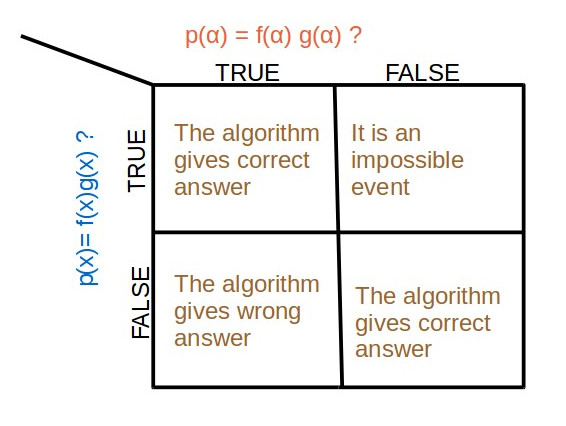
\includegraphics[width=0.6\textwidth]{confusion.jpg}
\label{confusion}
\caption{Possible Cases}
\end{figure}

As can be seen from Figure 1, the proposed algorithm gives incorrect result only in one of the cases, when the terms are actually not equal but our algorithm says that they are equal. \\

This happens when $\alpha$ is a root of the equation $\phi(x)=0$,or when $\alpha \in |S \cap R|$.  Hence, Probability (wrong answer)=\\

Pr ($\alpha \in |S \cap R|$)\\

= $\frac{|S \cap R|}{|S|}$\\

= $\frac{k}{10^d}$\\

$\leq$ $\frac{d}{10^d}$, since $k \leq d$\\

 
= $\frac{1}{10^d}$.

\textbf{Above algorithm runs in $O(d)$ time with probability of wrong answer = $\frac{1}{10^d}$ }



 
\end{document}